% Options for packages loaded elsewhere
\PassOptionsToPackage{unicode}{hyperref}
\PassOptionsToPackage{hyphens}{url}
%
\documentclass[
  ignorenonframetext,
]{beamer}
\usepackage{pgfpages}
\setbeamertemplate{caption}[numbered]
\setbeamertemplate{caption label separator}{: }
\setbeamercolor{caption name}{fg=normal text.fg}
\beamertemplatenavigationsymbolsempty
% Prevent slide breaks in the middle of a paragraph
\widowpenalties 1 10000
\raggedbottom
\setbeamertemplate{part page}{
  \centering
  \begin{beamercolorbox}[sep=16pt,center]{part title}
    \usebeamerfont{part title}\insertpart\par
  \end{beamercolorbox}
}
\setbeamertemplate{section page}{
  \centering
  \begin{beamercolorbox}[sep=12pt,center]{part title}
    \usebeamerfont{section title}\insertsection\par
  \end{beamercolorbox}
}
\setbeamertemplate{subsection page}{
  \centering
  \begin{beamercolorbox}[sep=8pt,center]{part title}
    \usebeamerfont{subsection title}\insertsubsection\par
  \end{beamercolorbox}
}
\AtBeginPart{
  \frame{\partpage}
}
\AtBeginSection{
  \ifbibliography
  \else
    \frame{\sectionpage}
  \fi
}
\AtBeginSubsection{
  \frame{\subsectionpage}
}
\usepackage{amsmath,amssymb}
\usepackage{lmodern}
\usepackage{iftex}
\ifPDFTeX
  \usepackage[T1]{fontenc}
  \usepackage[utf8]{inputenc}
  \usepackage{textcomp} % provide euro and other symbols
\else % if luatex or xetex
  \usepackage{unicode-math}
  \defaultfontfeatures{Scale=MatchLowercase}
  \defaultfontfeatures[\rmfamily]{Ligatures=TeX,Scale=1}
\fi
% Use upquote if available, for straight quotes in verbatim environments
\IfFileExists{upquote.sty}{\usepackage{upquote}}{}
\IfFileExists{microtype.sty}{% use microtype if available
  \usepackage[]{microtype}
  \UseMicrotypeSet[protrusion]{basicmath} % disable protrusion for tt fonts
}{}
\makeatletter
\@ifundefined{KOMAClassName}{% if non-KOMA class
  \IfFileExists{parskip.sty}{%
    \usepackage{parskip}
  }{% else
    \setlength{\parindent}{0pt}
    \setlength{\parskip}{6pt plus 2pt minus 1pt}}
}{% if KOMA class
  \KOMAoptions{parskip=half}}
\makeatother
\usepackage{xcolor}
\newif\ifbibliography
\usepackage{color}
\usepackage{fancyvrb}
\newcommand{\VerbBar}{|}
\newcommand{\VERB}{\Verb[commandchars=\\\{\}]}
\DefineVerbatimEnvironment{Highlighting}{Verbatim}{commandchars=\\\{\}}
% Add ',fontsize=\small' for more characters per line
\usepackage{framed}
\definecolor{shadecolor}{RGB}{248,248,248}
\newenvironment{Shaded}{\begin{snugshade}}{\end{snugshade}}
\newcommand{\AlertTok}[1]{\textcolor[rgb]{0.94,0.16,0.16}{#1}}
\newcommand{\AnnotationTok}[1]{\textcolor[rgb]{0.56,0.35,0.01}{\textbf{\textit{#1}}}}
\newcommand{\AttributeTok}[1]{\textcolor[rgb]{0.77,0.63,0.00}{#1}}
\newcommand{\BaseNTok}[1]{\textcolor[rgb]{0.00,0.00,0.81}{#1}}
\newcommand{\BuiltInTok}[1]{#1}
\newcommand{\CharTok}[1]{\textcolor[rgb]{0.31,0.60,0.02}{#1}}
\newcommand{\CommentTok}[1]{\textcolor[rgb]{0.56,0.35,0.01}{\textit{#1}}}
\newcommand{\CommentVarTok}[1]{\textcolor[rgb]{0.56,0.35,0.01}{\textbf{\textit{#1}}}}
\newcommand{\ConstantTok}[1]{\textcolor[rgb]{0.00,0.00,0.00}{#1}}
\newcommand{\ControlFlowTok}[1]{\textcolor[rgb]{0.13,0.29,0.53}{\textbf{#1}}}
\newcommand{\DataTypeTok}[1]{\textcolor[rgb]{0.13,0.29,0.53}{#1}}
\newcommand{\DecValTok}[1]{\textcolor[rgb]{0.00,0.00,0.81}{#1}}
\newcommand{\DocumentationTok}[1]{\textcolor[rgb]{0.56,0.35,0.01}{\textbf{\textit{#1}}}}
\newcommand{\ErrorTok}[1]{\textcolor[rgb]{0.64,0.00,0.00}{\textbf{#1}}}
\newcommand{\ExtensionTok}[1]{#1}
\newcommand{\FloatTok}[1]{\textcolor[rgb]{0.00,0.00,0.81}{#1}}
\newcommand{\FunctionTok}[1]{\textcolor[rgb]{0.00,0.00,0.00}{#1}}
\newcommand{\ImportTok}[1]{#1}
\newcommand{\InformationTok}[1]{\textcolor[rgb]{0.56,0.35,0.01}{\textbf{\textit{#1}}}}
\newcommand{\KeywordTok}[1]{\textcolor[rgb]{0.13,0.29,0.53}{\textbf{#1}}}
\newcommand{\NormalTok}[1]{#1}
\newcommand{\OperatorTok}[1]{\textcolor[rgb]{0.81,0.36,0.00}{\textbf{#1}}}
\newcommand{\OtherTok}[1]{\textcolor[rgb]{0.56,0.35,0.01}{#1}}
\newcommand{\PreprocessorTok}[1]{\textcolor[rgb]{0.56,0.35,0.01}{\textit{#1}}}
\newcommand{\RegionMarkerTok}[1]{#1}
\newcommand{\SpecialCharTok}[1]{\textcolor[rgb]{0.00,0.00,0.00}{#1}}
\newcommand{\SpecialStringTok}[1]{\textcolor[rgb]{0.31,0.60,0.02}{#1}}
\newcommand{\StringTok}[1]{\textcolor[rgb]{0.31,0.60,0.02}{#1}}
\newcommand{\VariableTok}[1]{\textcolor[rgb]{0.00,0.00,0.00}{#1}}
\newcommand{\VerbatimStringTok}[1]{\textcolor[rgb]{0.31,0.60,0.02}{#1}}
\newcommand{\WarningTok}[1]{\textcolor[rgb]{0.56,0.35,0.01}{\textbf{\textit{#1}}}}
\usepackage{longtable,booktabs,array}
\usepackage{calc} % for calculating minipage widths
\usepackage{caption}
% Make caption package work with longtable
\makeatletter
\def\fnum@table{\tablename~\thetable}
\makeatother
\usepackage{graphicx}
\makeatletter
\def\maxwidth{\ifdim\Gin@nat@width>\linewidth\linewidth\else\Gin@nat@width\fi}
\def\maxheight{\ifdim\Gin@nat@height>\textheight\textheight\else\Gin@nat@height\fi}
\makeatother
% Scale images if necessary, so that they will not overflow the page
% margins by default, and it is still possible to overwrite the defaults
% using explicit options in \includegraphics[width, height, ...]{}
\setkeys{Gin}{width=\maxwidth,height=\maxheight,keepaspectratio}
% Set default figure placement to htbp
\makeatletter
\def\fps@figure{htbp}
\makeatother
\setlength{\emergencystretch}{3em} % prevent overfull lines
\providecommand{\tightlist}{%
  \setlength{\itemsep}{0pt}\setlength{\parskip}{0pt}}
\setcounter{secnumdepth}{-\maxdimen} % remove section numbering
%% PDFメタデータの文字化け防止
% https://blog.miz-ar.info/2015/09/latex-hyperref-tips/
% https://tex.stackexchange.com/questions/24445/hyperref-lualatex-and-unicode-bookmarks-issue-garbled-page-numbers-in-ar-for-l
\hypersetup{%
  pdfencoding=auto
}

%% Fonts
\usefonttheme[onlymath]{serif}
\usepackage[T1]{fontenc}
\usepackage{textcomp}
%\usepackage{arev}
\usepackage[scale=1.0]{tgheros}  % San serif font
\usepackage[scaled]{beramono}    % Monospace font

%% Japanese font
\usepackage{luatexja-otf}
\usepackage[match,deluxe,expert,haranoaji,nfssonly]{luatexja-preset} % Notoフォント使用
\renewcommand{\kanjifamilydefault}{\gtdefault}

%%
\setbeamerfont{title}{size=\huge, series=\bfseries}
\setbeamerfont{frametitle}{size=\Large, series=\bfseries}

%% https://tex.stackexchange.com/questions/62202/change-background-colour-of-verbatim-environment
\let\oldv\verbatim
\let\oldendv\endverbatim
\def\verbatim{\par\setbox0\vbox\bgroup\oldv}
\def\endverbatim{\oldendv\egroup\fboxsep0pt \noindent\colorbox[gray]{0.95}{\usebox0}\par}

%% https://stackoverflow.com/questions/38323331/code-chunk-font-size-in-beamer-with-knitr-and-latex
%% change fontsize of R code
\let\oldShaded\Shaded
\let\endoldShaded\endShaded 
\renewenvironment{Shaded}{\footnotesize\oldShaded}{\endoldShaded}

\usepackage{listings}
\lstset{%
  frame = shadow,
  backgroundcolor = {\color[gray]{.95}},
  basicstyle = {\small\ttfamily},
  breaklines = true,
  upquote = true
}
%%%%%%%%%%%%%%%
\usepackage{booktabs}
\usepackage{tikz}
\usepackage{pxpgfmark} % remember picture を可能にする
\ifLuaTeX
  \usepackage{selnolig}  % disable illegal ligatures
\fi
\IfFileExists{bookmark.sty}{\usepackage{bookmark}}{\usepackage{hyperref}}
\IfFileExists{xurl.sty}{\usepackage{xurl}}{} % add URL line breaks if available
\urlstyle{same} % disable monospaced font for URLs
\hypersetup{
  pdfauthor={iotsuka},
  hidelinks,
  pdfcreator={LaTeX via pandoc}}

\title{oyoyo\\
hogehoge研修}
\author{iotsuka}
\date{2023-06-12}

\begin{document}
\frame{\titlepage}

\begin{frame}{a beautiful story}
\protect\hypertarget{a-beautiful-story}{}
\Huge

\begin{itemize}[<+->]
\tightlist
\item
  \textbullet{}\hspace{3pt}予算の会議
\item
  \textbullet{}\hspace{3pt}ある事業について
\item
  \textbullet{}\hspace{3pt}どんな成果?
\end{itemize}
\end{frame}

\begin{frame}{a beautiful story}
\protect\hypertarget{a-beautiful-story-1}{}
\IfFileExists{kids.jpg}{\centering\includegraphics{kids.jpg}}{\relax}
\end{frame}

\begin{frame}{evidence-based policy-making}
\protect\hypertarget{evidence-based-policy-making}{}
\Huge

\begin{itemize}[<+->]
\tightlist
\item
  \textbullet{}\hspace{3pt}思いだけでは進まない \bigskip
\item
  \textbullet{}\hspace{3pt}客観的な根拠 \bigskip
\item
  \mbox{}\hfill{}{\textrightarrow{}\,\,{}}dataの活用
\end{itemize}
\end{frame}

\begin{frame}{quiz:whaddayathink?}
\protect\hypertarget{quizwhaddayathink}{}
\Huge

検査を受けました\pause{\textrightarrow{}\,\,{}陽性!!!}
\end{frame}

\begin{frame}{quiz:whaddayathink?}
\protect\hypertarget{quizwhaddayathink-1}{}
\LARGE

\begin{itemize}
\item どんな病気??
\pause
\item  \textbullet{}\hspace{2pt}1\%の人がこの病気にかかってる
\pause
\item 
\item どんな検査??
\pause
\item  \textbullet{}\hspace{2pt}病気なら90\%の確率で陽性
\pause
\item  \textbullet{}\hspace{2pt}病気でないなら90\%の確率で陰性
\end{itemize}
\end{frame}

\begin{frame}{quiz:whaddayathink?}
\protect\hypertarget{quizwhaddayathink-2}{}
\Huge

実際に病気である確率は??
\end{frame}

\begin{frame}{tree}
\protect\hypertarget{tree}{}
\scalebox{.88}{%
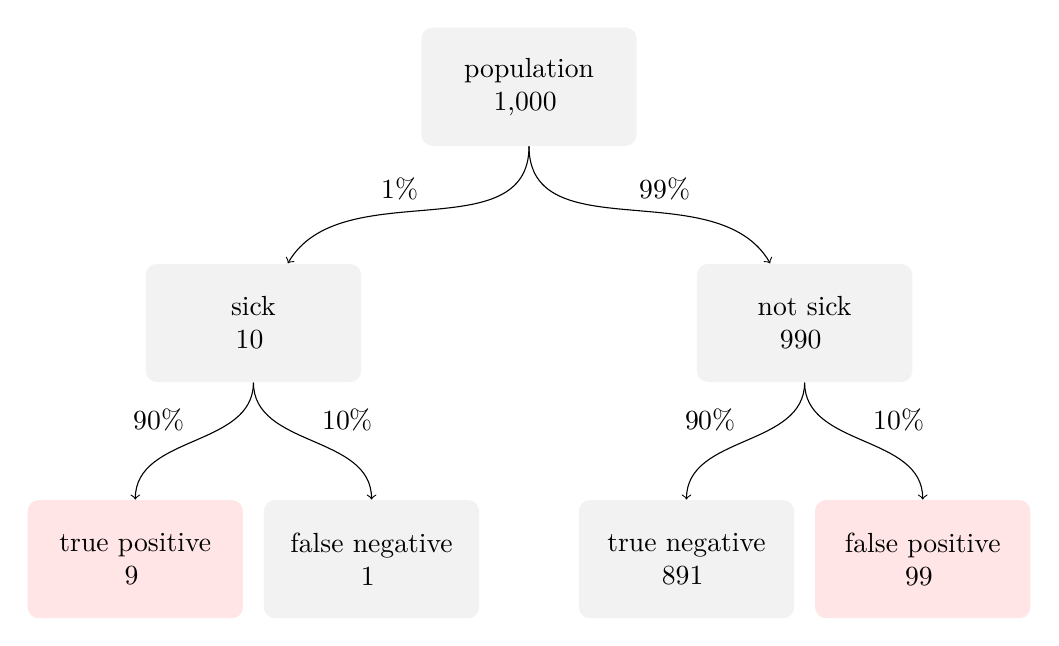
\begin{tikzpicture}
 \tikzset{block/.style={rectangle, text width=25mm, text centered, rounded corners, minimum height=1.5cm}};
%\draw [help lines] (-6,0) grid (6,6);%(0,0)から(10,4)までの"細線の方眼"
\node[block,fill=gray!10] (population) at (0,7) {population\\1,000人};
\pause
\node[block,fill=gray!10] (sick) at (-3.5,4) {sick\\10人};
\draw [->] (population) to[out=-90, in=60] node[auto=right] {$1\%$} (sick); 
\pause
\node[block,fill=gray!10] (not_sick) at (3.5,4) {not sick\\990人};
\draw [->] (population) to[out=-90, in=120]  node[auto=left] {$99\%$} (not_sick); 
\pause
\node[block,fill=red!10] (true_positive) at (-5,) {true positive\\9人};
\draw [->] (sick) to[out=-90, in=90]  node[auto=right] {$90\%$} (true_positive); 
\pause
\node[block,fill=gray!10] (false_negative) at (-2,1) {false negative\\1人};
\draw [->] (sick) to[out=-90, in=90]  node[auto=left] {$10\%$} (false_negative); 
\pause
\node[block,fill=gray!10] (true_negative) at (2,1) {true negative\\891人};
\draw [->] (not_sick) to[out=-90, in=90]  node[auto=right] {$90\%$} (true_negative); 
\pause
\node[block,fill=red!10] (false_positive) at (5,1) {false positive\\99人};
\draw [->] (not_sick) to[out=-90, in=90]  node[auto=left] {$10\%$} (false_positive); 
 \end{tikzpicture}%
}
\end{frame}

\begin{frame}{answer}
\protect\hypertarget{answer}{}
\begin{center}\Huge
\[
\frac{9}{9 + 99}=0.083333
\ldots
\]
\end{center}
\end{frame}

\begin{frame}{world war II}
\protect\hypertarget{world-war-ii}{}
\raggedleft
\IfFileExists{survivorship_bias.png}{\scalebox{.9}{\includegraphics{survivorship_bias.png}}}{\relax}

\tiny

\raggedleft

Martin Grandjean(vector), McGeddon(picture), Cameron Moll(concept)

\vspace{-5pt}

This work is licensed under the Creative Commons Attribution-Share Alike
4.0 International license.
\end{frame}

\begin{frame}{research}
\protect\hypertarget{research}{}
\LARGE

\begin{itemize}[<+->]
\tightlist
\item
  \textbullet ある町
\item
  \textbullet\hspace{1pt} 4つの学校
\item
  \textbullet 同じテスト
\end{itemize}
\end{frame}

\begin{frame}{research}
\protect\hypertarget{research-1}{}
\LARGE

\begin{itemize}[<+->]
\tightlist
\item
   \textbullet 家庭での学習時間
\item
   \textbullet 正答率
\end{itemize}
\end{frame}

\begin{frame}{hypothethis}
\protect\hypertarget{hypothethis}{}
\LARGE

学習時間と正答率に関係はあるのか??
\end{frame}

\begin{frame}{plot}
\protect\hypertarget{plot}{}
\includegraphics{slide_files/figure-beamer/unnamed-chunk-6-1.pdf}
\end{frame}

\begin{frame}{plot}
\protect\hypertarget{plot-1}{}
\includegraphics{slide_files/figure-beamer/unnamed-chunk-7-1.pdf}
\end{frame}

\begin{frame}{plot}
\protect\hypertarget{plot-2}{}
\IfFileExists{./letsnotsee.jpg}{\includegraphics[width=\textwidth]{./letsnotsee.jpg}}{\relax}
\end{frame}

\begin{frame}{plot}
\protect\hypertarget{plot-3}{}
\includegraphics{slide_files/figure-beamer/unnamed-chunk-8-1.pdf}
\end{frame}

\begin{frame}{plot}
\protect\hypertarget{plot-4}{}
\includegraphics{slide_files/figure-beamer/unnamed-chunk-9-1.pdf}
\end{frame}

\begin{frame}{plot}
\protect\hypertarget{plot-5}{}
\includegraphics{slide_files/figure-beamer/unnamed-chunk-10-1.pdf}
\end{frame}

\begin{frame}{plot}
\protect\hypertarget{plot-6}{}
\includegraphics{slide_files/figure-beamer/unnamed-chunk-11-1.pdf}
\end{frame}

\begin{frame}{plot}
\protect\hypertarget{plot-7}{}
\includegraphics{slide_files/figure-beamer/unnamed-chunk-12-1.pdf}
\end{frame}

\begin{frame}{Simpson's Paradox}
\protect\hypertarget{simpsons-paradox}{}
\LARGE

\begin{itemize}[<+->]
\tightlist
\item
  \textbullet{}\hspace{2pt}全体では

  \par

  「勉強するほど成績がさがる」 \bigskip
\item
  \textbullet{}\hspace{2pt}学校ごとでは

  \par

  「勉強するほど成績があがる」
\end{itemize}

\normalsize
\end{frame}

\begin{frame}{tebiki}
\protect\hypertarget{tebiki}{}
\vspace*{-20pt}
\IfFileExists{./tebiki.jpg}{\centering\scalebox{.9}{\rotatebox{-90}{\includegraphics[width=\textheight]{tebiki.jpg}}}}{\relax}
\end{frame}

\begin{frame}{Sir Winston Spencer Churchill}
\protect\hypertarget{sir-winston-spencer-churchill}{}
\raggedleft\Huge

\raisebox{100pt}{\rotatebox{30}{\textcolor{white}{Brevity}}}  
\IfFileExists{Sir_Winston_Churchil.jpg}{\scalebox{.75}{\includegraphics{Sir_Winston_Churchil.jpg}}}{\relax}

\tiny

\raggedleft

The Roaring Lion(Yousuf Karsh) \vspace{-5pt}

This work is licensed under the Creative Commons Attribution 2.0 Generic
License.
\end{frame}

\begin{frame}{Sir Winston Spencer Churchill}
\protect\hypertarget{sir-winston-spencer-churchill-1}{}
\raggedleft\Huge

\raisebox{100pt}{\rotatebox{30}{\textcolor{black}{Brevity}}}  
\IfFileExists{Sir_Winston_Churchil.jpg}{\scalebox{.75}{\includegraphics{Sir_Winston_Churchil.jpg}}}{\relax}

\tiny

\raggedleft

The Roaring Lion(Yousuf Karsh) \vspace{-5pt}

This work is licensed under the Creative Commons Attribution 2.0 Generic
License.
\end{frame}

\begin{frame}{Brevity}
\protect\hypertarget{brevity}{}
\centering
\vspace*{-21.5pt}
\IfFileExists{churchill_memo.jpg}{\scalebox{1.025}{\includegraphics{churchill_memo.jpg}}}{\relax}
\end{frame}

\begin{frame}{Brevity}
\protect\hypertarget{brevity-1}{}
\Large

To do our work, we all have to read a mass of papers. Nearly all of them
are far too long.

\par

\vfill
\Huge

\rotatebox{15}{\scalebox{1.6}{\textcolor{white}{\begin{tabular}{l}大量の書類\\長すぎる\end{tabular}}}}

\vfill
\end{frame}

\begin{frame}{Brevity}
\protect\hypertarget{brevity-2}{}
\Large

To do our work, we all have to read \textcolor{olive}{a mass of papers}.
Nearly all of them are \textcolor{olive}{far too long}.

\par

\vfill
\Huge

\rotatebox{15}{\scalebox{1.6}{\textcolor{olive}{\begin{tabular}{l}大量の書類\\長すぎる\end{tabular}}}}

\vfill
\end{frame}

\begin{frame}{Brevity}
\protect\hypertarget{brevity-3}{}
\Large

This wastes time, while energy has to be spent in looking for the
essential points.

\par

\vfill\Huge

\rotatebox{15}{\scalebox{1.6}{\textcolor{white}{\begin{tabular}{l}時間のむだ\\要点がわからない\end{tabular}}}}

\vfill
\end{frame}

\begin{frame}{Brevity}
\protect\hypertarget{brevity-4}{}
\Large

This \textcolor{olive}{wastes time}, while energy has to be spent in
looking for \textcolor{olive}{the essential points}.

\par

\vfill\Huge

\rotatebox{15}{\scalebox{1.6}{\textcolor{olive}{\begin{tabular}{l}時間のむだ\\要点がわからない\end{tabular}}}}

\vfill
\end{frame}

\begin{frame}{Brevity}
\protect\hypertarget{brevity-5}{}
\Large

I ask my colleagues and their staffs to see to it that their Reports are
shorter.

\vfill\Huge

\rotatebox{15}{\scalebox{1.6}{\textcolor{white}{\begin{tabular}{l}報告書を短く\end{tabular}}}}

\vfill
\end{frame}

\begin{frame}{Brevity}
\protect\hypertarget{brevity-6}{}
\Large

I ask my colleagues and their staffs to see to it that
\textcolor{olive}{their Reports are shorter}.

\vfill\Huge

\rotatebox{15}{\scalebox{1.6}{\textcolor{olive}{\begin{tabular}{l}報告書を短く\end{tabular}}}}

\vfill
\end{frame}

\begin{frame}{Brevity}
\protect\hypertarget{brevity-7}{}
\Large

\begin{itemize}
 \item[\textbullet] 歯切れよく言い切れ
 \item[\textbullet] もってまわったいいまわしはやめろ
 \item[\textbullet] 詳細な分析は付録にしろ
 \item[\textbullet] 見出しだけのメモ---口頭で補うのもあり
 \item[\textbullet] 乱暴な表現でかまわない
\end{itemize}
\end{frame}

\begin{frame}{what is important}
\protect\hypertarget{what-is-important}{}
\Huge

\begin{itemize}[<+->]
\tightlist
\item
  \textbullet{}\hspace{2pt}本質的なこと \bigskip
\item
  \textbullet{}\hspace{2pt}体裁 \bigskip
\item
  \textbullet{}\hspace{2pt}スピード感
\end{itemize}
\end{frame}

\begin{frame}{tebiki}
\protect\hypertarget{tebiki-1}{}
\vspace*{-20pt}
\IfFileExists{./tebiki.jpg}{\centering\scalebox{.9}{\rotatebox{-90}{\includegraphics[width=\textheight]{tebiki.jpg}}}}{\relax}
\end{frame}

\begin{frame}{quiz}
\protect\hypertarget{quiz}{}
\Huge

\begin{itemize}[<+->]
\tightlist
\item
  「又は」or「または」 \bigskip
\item
  「子供」or「子ども」 \bigskip
\item
  「手引」or「手引き」
\end{itemize}
\end{frame}

\begin{frame}{attraction}
\protect\hypertarget{attraction}{}
\vspace*{-4pt}
\IfFileExists{./bento.jpg}{\centering\scalebox{.85}{\includegraphics[width=\textheight]{bento.jpg}}}{\relax}
\end{frame}

\begin{frame}{last but not least}
\protect\hypertarget{last-but-not-least}{}
\end{frame}

\begin{frame}{data}
\protect\hypertarget{data}{}
\begin{itemize}[<+->]
\item
  4つのデータ(data\_1 ~ data\_4)があります
\item
  それぞれのデータは、11組のxとyから構成されています
\end{itemize}
\end{frame}

\begin{frame}{data}
\protect\hypertarget{data-1}{}
\begin{tabular}{rr}
\multicolumn{2}{l}{data\_1}\\
\toprule
x & y\\
\midrule
10 & 8.04\\
8 & 6.95\\
13 & 7.58\\
9 & 8.81\\
11 & 8.33\\
14 & 9.96\\
6 & 7.24\\
4 & 4.26\\
12 & 10.84\\
7 & 4.82\\
5 & 5.68\\
\bottomrule
\end{tabular}\hfill
\begin{tabular}{rr}
\multicolumn{2}{l}{data\_2}\\
\toprule
x & y\\
\midrule
10 & 9.14\\
8 & 8.14\\
13 & 8.74\\
9 & 8.77\\
11 & 9.26\\
14 & 8.10\\
6 & 6.13\\
4 & 3.10\\
12 & 9.13\\
7 & 7.26\\
5 & 4.74\\
\bottomrule
\end{tabular}\hfill
\begin{tabular}{rr}
\multicolumn{2}{l}{data\_3}\\
\toprule
x & y\\
\midrule
10 & 7.46\\
8 & 6.77\\
13 & 12.74\\
9 & 7.11\\
11 & 7.81\\
14 & 8.84\\
6 & 6.08\\
4 & 5.39\\
12 & 8.15\\
7 & 6.42\\
5 & 5.73\\
\bottomrule
\end{tabular}\hfill
\begin{tabular}{rr}
\multicolumn{2}{l}{data\_4}\\
\toprule
x & y\\
\midrule
8 & 6.58\\
8 & 5.76\\
8 & 7.71\\
8 & 8.84\\
8 & 8.47\\
8 & 7.04\\
8 & 5.25\\
19 & 12.50\\
8 & 5.56\\
8 & 7.91\\
8 & 6.89\\
\bottomrule
\end{tabular}
\end{frame}

\begin{frame}{data}
\protect\hypertarget{data-2}{}
それぞれどういうデータなんだろう

\begin{itemize}[<+->]
\tightlist
\item
  表だけ見てもよくわからない
\end{itemize}
\end{frame}

\begin{frame}{data}
\protect\hypertarget{data-3}{}
それぞれどういうデータなんだろう

\begin{itemize}[<+->]
\tightlist
\item
  xの平均
\item
  xの分散
\item
  yの平均
\item
  yの分散
\item
  xとyの相関係数
\item
  回帰直線の式
\end{itemize}
\end{frame}

\begin{frame}{summarise}
\protect\hypertarget{summarise}{}
\begin{longtable}[]{@{}lrrrrr@{}}
\toprule()
data & x\_mean & x\_var & y\_mean & y\_var & cor \\
\midrule()
\endhead
data\_1 & 9 & 11 & 7.500909 & 4.127269 & 0.8164205 \\
data\_2 & 9 & 11 & 7.500909 & 4.127629 & 0.8162365 \\
data\_3 & 9 & 11 & 7.500000 & 4.122620 & 0.8162867 \\
data\_4 & 9 & 11 & 7.500909 & 4.123249 & 0.8165214 \\
\bottomrule()
\end{longtable}

\begin{itemize}
\tightlist
\item
  要約統計量はよく似ている
\end{itemize}
\end{frame}

\begin{frame}[fragile]{visualization}
\protect\hypertarget{visualization}{}
\begin{figure}
\centering
\includegraphics{slide_files/figure-beamer/unnamed-chunk-15-1.pdf}
\caption{\texttt{ggplot2} によるグラフ}
\end{figure}
\end{frame}

\begin{frame}[fragile]{visualization}
\protect\hypertarget{visualization-1}{}
\begin{figure}
\centering
\includegraphics{slide_files/figure-beamer/unnamed-chunk-16-1.pdf}
\caption{\texttt{ggplot2} によるグラフ}
\end{figure}
\end{frame}

\begin{frame}{lesson}
\protect\hypertarget{lesson}{}
表でみてもよくわからない

平均値とか分散を計算してもよくわからない

図示がだいじ
\end{frame}

\begin{frame}{quiz:How many millions are in a trillion?}
\protect\hypertarget{quizhow-many-millions-are-in-a-trillion}{}
\includegraphics{slide_files/figure-beamer/unnamed-chunk-17-1.pdf}
\end{frame}

\begin{frame}{quiz:How many millions are in a trillion?}
\protect\hypertarget{quizhow-many-millions-are-in-a-trillion-1}{}
\LARGE

1兆は100万の何倍でしょう?

\begin{tabular}{rr}\toprule
回答&率\\\midrule
千倍&18\%\\
万倍&12\%\\
10万倍&21\%\\
100万倍&21\%\\
1000万倍&17\%\\
わからない&12\%\\\bottomrule
\end{tabular}
\end{frame}

\begin{frame}{pie chart}
\protect\hypertarget{pie-chart}{}
\includegraphics[height=8cm]{slide_files/figure-beamer/unnamed-chunk-19-1}
\end{frame}

\begin{frame}{substitute for a pie chart}
\protect\hypertarget{substitute-for-a-pie-chart}{}
\includegraphics{slide_files/figure-beamer/unnamed-chunk-20-1.pdf}
\end{frame}

\begin{frame}{substitute for a pie chart}
\protect\hypertarget{substitute-for-a-pie-chart-1}{}
\includegraphics{slide_files/figure-beamer/unnamed-chunk-21-1.pdf}
\end{frame}

\begin{frame}[fragile]{substitute for a pie chart}
\protect\hypertarget{substitute-for-a-pie-chart-2}{}
\begin{verbatim}
## Warning: Using `size` aesthetic for lines was deprecated in ggplot2 3.4.0.
## i Please use `linewidth` instead.
## This warning is displayed once every 8 hours.
## Call `lifecycle::last_lifecycle_warnings()` to see where this warning was
## generated.
\end{verbatim}

\includegraphics{slide_files/figure-beamer/unnamed-chunk-22-1.pdf}
\end{frame}

\begin{frame}{quiz:How many millions are in a trillion?}
\protect\hypertarget{quizhow-many-millions-are-in-a-trillion-2}{}
\includegraphics{slide_files/figure-beamer/unnamed-chunk-23-1.pdf}
\end{frame}

\begin{frame}[fragile]{Slide with R Output}
\protect\hypertarget{slide-with-r-output}{}
\begin{Shaded}
\begin{Highlighting}[]
\FunctionTok{summary}\NormalTok{(cars)}
\end{Highlighting}
\end{Shaded}

\begin{verbatim}
##      speed           dist       
##  Min.   : 4.0   Min.   :  2.00  
##  1st Qu.:12.0   1st Qu.: 26.00  
##  Median :15.0   Median : 36.00  
##  Mean   :15.4   Mean   : 42.98  
##  3rd Qu.:19.0   3rd Qu.: 56.00  
##  Max.   :25.0   Max.   :120.00
\end{verbatim}
\end{frame}

\begin{frame}{文書・資料}
\protect\hypertarget{ux6587ux66f8ux8cc7ux6599}{}
\begin{itemize}[<+->]
\tightlist
\item
  \textbullet{}\hspace{2pt} The aim should be Reports which set out the
  main points in a series of short, crisp paragraphs.
\item
  \textbullet{}\hspace{2pt} If a Report relies on detailed analysis of
  some complicated factors, or on statistics, these should be set out in
  an Appendix.
\item
  \textbullet{}\hspace{2pt} Often the occasion is best met by submitting
  not a full-dress Report, but an Aide-memoire consisting of headings
  only, which can be expanded orally if needed.
\item
  \textbullet\hspace{2pt}Let us have an end of such phrases as these:
  ``It is also of importance to bear in mind the following
  considerations\ldots{}'', or ``Consideration should be given to the
  possibility of carrying into effect\ldots{}'' Most of these woolly
  phrases are mere padding, which can be left out altogether, or
  replaced by a single word. Let us not shrink from using the short
  expressive phrase, even if it is conversational.
\end{itemize}
\end{frame}

\begin{frame}{文書・資料}
\protect\hypertarget{ux6587ux66f8ux8cc7ux6599-1}{}
Reports drawn up on the lines I propose may at first seem rough as
compared with the flat surface of officialese jargon. But the saving in
time will be great, while the discipline of setting out the real points
concisely will prove an aid to clearer thinking.
\end{frame}

\begin{frame}{tohoho}
\protect\hypertarget{tohoho}{}
\includegraphics{slide_files/figure-beamer/unnamed-chunk-26-1.pdf}
\end{frame}

\begin{frame}[fragile]{tohoho}
\protect\hypertarget{tohoho-1}{}
\includegraphics{slide_files/figure-beamer/unnamed-chunk-27-1.pdf}

\begin{block}{誕生日問題}
\protect\hypertarget{ux8a95ux751fux65e5ux554fux984c}{}
閏年は無視。 k人の集団で同じ誕生日の人がいるかどうか。

\begin{block}{少なくとも1組はいる確率}
\protect\hypertarget{ux5c11ux306aux304fux3068ux30821ux7d44ux306fux3044ux308bux78baux7387}{}
\begin{verbatim}
##  [1] 0.000 0.000 0.004 0.018 0.022 0.044 0.063 0.080 0.083 0.130 0.134 0.173
## [13] 0.212 0.239 0.236 0.270 0.313 0.352 0.361 0.407 0.438 0.486 0.468 0.534
## [25] 0.586 0.603 0.643 0.651 0.683 0.695 0.717 0.755 0.775 0.788 0.821 0.819
## [37] 0.851 0.861 0.868 0.891
\end{verbatim}
\end{block}

\begin{block}{同じ誕生日の}
\protect\hypertarget{ux540cux3058ux8a95ux751fux65e5ux306e}{}
\begin{verbatim}
##  [1] 0.000 0.001 0.009 0.014 0.024 0.028 0.053 0.079 0.116 0.119 0.151 0.177
## [13] 0.228 0.248 0.282 0.313 0.369 0.405 0.469 0.545 0.595 0.605 0.676 0.711
## [25] 0.827 0.872 0.931 0.989 1.095 1.258 1.206 1.256 1.398 1.456 1.558 1.717
## [37] 1.780 1.874 1.960 2.107
\end{verbatim}
\end{block}
\end{block}
\end{frame}

\end{document}
